
\documentclass[11pt,a4paper,twoside]{article}

\usepackage[numbers, authoryear]{natbib}
\usepackage{url}
\usepackage{parskip}
\usepackage{graphicx}

\setlength{\oddsidemargin}{-0.4mm} % 25 mm left margin
\setlength{\evensidemargin}{\oddsidemargin}
\setlength{\textwidth}{160mm}      % 25 mm right margin
\setlength{\topmargin}{-5.4mm}     % 20 mm top margin
\setlength{\headheight}{5mm}
\setlength{\headsep}{5mm}
\setlength{\footskip}{10mm}
\setlength{\textheight}{237mm}     % 20 mm bottom margin
\setlength{\parindent}{12pt}
\begin{document}

\setcounter{page}{1}

\title{Implementing a Personal Container}
\author{Chris Elsmore}
%\date{} % do not add a date1
\date{October 2011}

\maketitle % optional

\begin{abstract}
This document explains the motivation behind setting up a personal container style data store, and the advantages such a container can provide. Online services are becoming increasingly popular and more numerous, however with this growth comes greater scattering of personal data. We discuss using a Personal Container allows this data to be stored where the user chooses, in the cloud or on a computer at home, in the first instance preventing data loss resulting from the closure of an online service, and in the second allowing a user to more closely allow or deny access to their data, along with letting third parties run algorithms on their personal container and return results without exposing the raw information. Using an implementation of the Personal Container paradigm called Locker, we can setup infrastructure internally, and use it to provide detailed information to a user based on their personal and sensitive data without exposing the raw data and compromising privacy. We show an example of this infrastructure by deploying it within the University as a pilot study, to identify the benefits both to employees who can use the container to store information, and the university that can request access to this information for surveys, and future decision making.
\end{abstract}

\newpage
% \tableofcontents % optional
%\section{Introduction}

\section{Motivation}

\subsection{Current Practice \& Limitations}
Online services and social networking websites have surged in popularity and now enjoy vast user bases - Facebook currently has 800 Million active users\cite{facebook:qr}, and Foursquare has acquired 100 Million Users in its 27 month lifetime\cite{foursquare:sd}. These sites store a significant amount of user generated content - members upload 8 years worth of video using YouTube, 250 million photos to Facebook and generate over 200 million tweets on Twitter each day\cite{youtube:sa},\cite{twiter:st}.

The users who generate this data must trust that these sites will continue to exist to continue accessing this content. In the case of photo sharing sites the user most likely has copies of the images they have uploaded elsewhere, but does not have their own copy of the metadata generated after upload -for example conversations regarding photos. Sites like Twitter and Foursquare by their nature don't generate any data locally, and all tweet and checkin data is stored remotely by the service. If these sites were to disappear, users would not have access to their own data without manually backing up beforehand, often using custom code using an API, a high barrier of entry for the non-technical user.

Even if users are technically savvy and willing to write code or trust 3rd party applications that access data on their behalf, users with a wide reaching digital footprint will require many different apps accessing many different API endpoints to reach their data, all with their own idiosyncratic behaviour within standards such as OAuth\footnote{More information available at \url{http://oauth.net/}}, used for authentication. Access to this data is further burdened by the use of certain 3rd party applications which in the case of sites such as Facebook, have been known to have security and privacy concerns \cite{consumerist:sa} \cite{ZDnet:cs} \cite{wsj:sa} \cite{eff:sa}.


\newpage
\section{Personal Containers}

\subsection{Description}
Personal Containers are designed to solve the problem of fragmentation of user data throughout the social web, compute additional, higher resolution and more accurate personal data by combining multiple data sources, and facilitate tighter security around access to these data. They are basic data storage and access systems, and can range from simple databases of information on a single computer hosted by the user, to sophisticated systems that act as signposts, storing the location of all user data on multiple devices and services, and proxying requests to the relevant data sources.



\subsection{Benefits}

Personal Containers provide a central access point to and allow autonomous collection of a users data from multiple sources, with data such as photos, tweets, status updates, checkins etc. Since the container provides direct access to multiple sources of data, it is able to generate far higher resolution data than using data from just one service- for example using geo-tagged tweets, photos and checkins along with Google Latitude\footnote{More information available at \url{http://google.com/latitude/}} data to provide highly accurate location information. It also allows faster and simpler access to multiple data, enable simple queries such as requesting all photos taken between two dates.

Personal Containers also ofter the possibility of increased security and data control. Personal data is by definition personal, and thus highly sensitive. The examples above demonstrate the need to added security, when dealing with highly accurate and real-time location data for example. The personal container can use multiple factors to approve or deny requests based on traditional variables such as rate of access, and simple authentication, as well as time based restrictions such as validity windows where data access is only allowed for a certain time, and impose certain restrictions based on media type such as picture or location resolution.The container can also allow results based on computation on personal container data to be accessed without allowing direct access to the data itself, instead taking in an algorithm to run, and returning a result based on that algorithm instead of raw data. 

The data security befits are not only a matter of authentication; personal containers can act as sophisticated backup mechanisms of sensitive data, de-duplicating and federating throughout storage nodes such as personal computers at a users home or workplace, or instances running on cloud computing platforms such as Amazon's EC2\footnote{More information available at \url{http://aws.amazon.com/ec2/}}.


\newpage
\section{Implementation}

\subsection{Architecture}
The Locker Project\footnote{More information available at \url{http://lockerproject.org/}} aims to construct a personal container suitable for hosting on a users personal computer, as well as adapting to a cloud based platform or a dedicated machine hosted personally. It is written in Javascript on the Node.js\footnote{More information available at \url{http://nodejs.org/}} platform for the backend, HTML and Javascript on the web-based user interface, and uses a MongoDB\footnote{More information available at \url{http://www.mongodb.org/}} database for data storage.

\begin{figure}[h]
  \begin{center}
    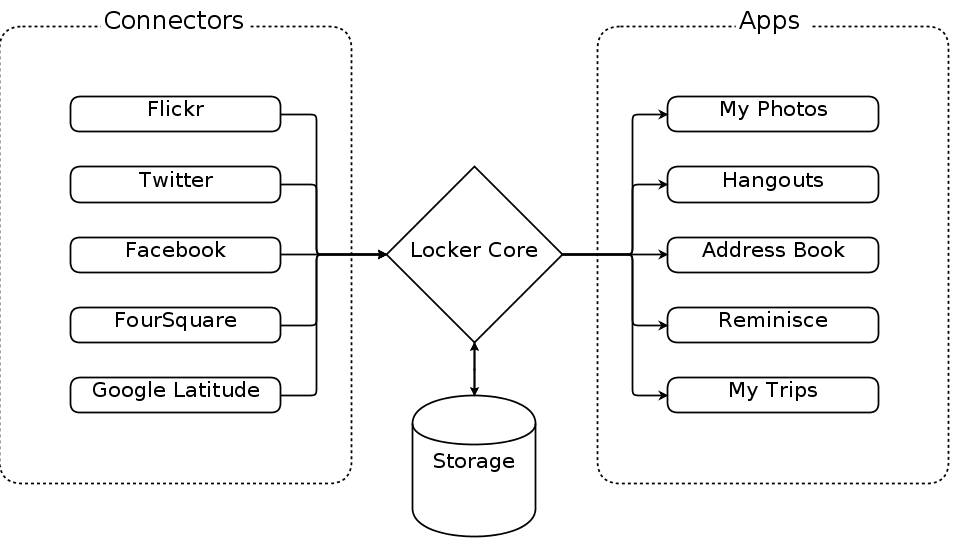
\includegraphics[scale=0.4]{LockerDia.png}
  \end{center}
  \caption{Architecture of the Locker platform.}
  \label{img-lockerDia}
\end{figure}

As figure \ref{img-lockerDia} explains, the Locker platform is made up from 4 main components. Connectors are responsible for connecting to and downloading data from endpoints such as Flickr or Facebook, and presenting this data to the Locker Core. Core is the central Locker process that fires events such as checking and updating the personal data stored in the Locker, or handling data search queries. Core can start and end connector and app processes which intercommunicate using JSON, and is also responsible for placing and retrieving data in the database. It also provides a query API to the stored data, which the apps can use to retrieve and display data to the user.

\newpage
\subsection{Infrastructure}
Our deployment infrastructure involves multiple instances of the locker platform, installed on multiple virtual machines running a Linux OS with a secure proxy frontend. The locker codebase supports only single users with no authentication, so each instance is isolated within it's own virtual machine. A central Nginx\footnote{More information available at \url{http://nginx.org/}} server handles SSL encryption, authentication and acts as a proxy to direct the user to the correct instance based on the hostname requested internally to the host machine.

The deployment is hosted by the university cloud computing service, as an example of an institution hosting secure personal data storage, in return for access to said data in an open, and transparent way, identifying to the user exactly which data will be used, and for what purpose.

\subsection{Advantages}


\begin{figure}[h]
  \begin{center}
    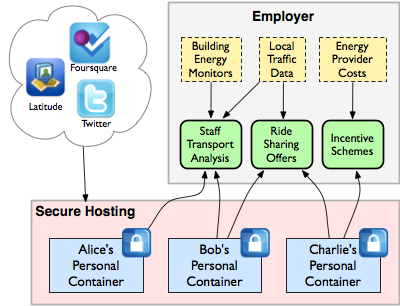
\includegraphics[scale=0.8]{PersConDataflow.png}
  \end{center}
  \caption{C-Aware Personal Container deployment layout and possible schemes.}
  \label{img-persConDia}
\end{figure}

As shown in figure \ref{img-persConDia}, using this system an employer can offer a range of schemes to it's employees, as well as using this data for it's own projects, in a privacy preserving way, and with the explicit permission of the users.

\newpage

\subsection{Deployment Scenarios}

There are numerous deployment scenarios that the University could use to provide rich services to both itself and it's users, with two such possibilities are documented below.

Both require the University to install the infrastructure discussed earlier as a University wide service. Signing up to the service would authenticate users against a university database, and grant access whilst setting up a new blank locker for the user to use. The user can then add their own data by enabling various connectors to pull in personal data from social networking websites and the like, as well as the university's custom connectors for location tracking, building energy use etc. This data can then be requested via the University for differing ends, and in different ways, which can primarily benefit the user, the university or both.

\subsubsection{Staff Transport Analysis}

The University currently conducts travel to work surveys to gather data about how it's staff are commuting to their place of work, how long they are taking and where they are traveling to and from\footnote{More information available at \url{http://www.admin.cam.ac.uk/offices/em/travel/}}. This data is used for future planning of university infrastructure such as car parks, bike racks, and cycle lanes, as well as communicated to the local council to plan road, bus and cycle network improvements that help to ease congestion and improve safety. The data is also used to calculate how much of an impact university staff have on the environment via the carbon output of their chosen transport methods, and to assist planning efforts to reduce this\cite{rserg:sfg}.

Asking users to allow the University access to their location data from such services as Google Latitude and Foursquare enables the University to use this data to infer the habits of it's staff without having them fill out a survey, or rely on data that may not be accurate as it relies on respondents memory. It also prevents spoilt returns - in the 2010 survey, 203 returns were spoilt and could not be used, ~�2\% of the surveys completed \cite{rserg:8drg6}.

The data available to the University can be augmented by using a Travel To Work app installable on users smartphones. This app can be used to record the users location with high accuracy and resolution, and store it in the users personal container. This additional data can be used to increase the accuracy of the location data already in the locker, and used to gather data on exact routes to work, as well as combined with traffic data and bus routes to predict what method of transport was being used.

This high resolution data has serious privacy implications, but the privacy inherent in the architecture prevents access to the data that the user does not grant. The travel to work app can be set with the users rough commuting times, to prevent other non-commute related travel data being recorded at other times of the day. It can also allow easily shutting off the location tracking, as well as retroactively erasing recorded data in the locker. Furthermore the data can be analysed within the locker by the user and erased if desired,  and the data that the University is allowed to access could be limited by time or location, thus the user can indicate a typical commute route, and prevent access to data that deviates significantly from this route.

Additional data contained within the locker could be used to recommend friends on social networks that take a route to work similar to a users own, to offer carpooling, or cycling in a group etc. The university could also provide pointers to modifying your route to work, suggesting faster or safer alternatives.

\subsubsection{Financial Offers}

The University could also offer financial benefits to it's users through the data store in the locker. Using a connector to a users home energy meter, the locker can store high resolution gas and electricity consumption information, to inform the user of their usage habits. This can be expanded in many ways, such as using multiple energy monitors on individual appliances and offering recommendations for newer more efficient devices, or using the historical usage data to recommend energy tariffs that are cheaper based on recorded usage without the user having to find old bills.

With such data available, the University could also start offering sophisticated services that add awareness to existing schemes and services. For example calculating how much money a user spends using a car during their commute, and indicating the payback time of using the Cycle to Work Scheme\footnote{More information available at \url{http://www.admin.cam.ac.uk/offices/hr/staff/benefits/cycle/}} to buy a bicycle through salary sacrifice, including when the user breaks even and becomes better off.

As discussed above, the data involved in these services is directly controlled by the user, each service will stipulate exactly what data it needs and why, and they can revoke access at any time. We believe this control coupled with the possibility of hosting lockers as appliances within users own homes, or on cloud platforms they trust including the university's, will result in the majority of users being happy to store their personal data in such a container as the benefits are not only convenience but also financial.


\newpage
\bibliographystyle{abbrv}
\renewcommand{\bibname}{References} % changes default name Bibliography to References
\bibliography{LockerTechReport} % References file
%\addcontentsline{toc}{chapter}{References} %adds References to contents page

\end{document}